\documentclass[12pt]{article}
\renewcommand{\baselinestretch}{1.4}
\usepackage{graphicx}

\usepackage[light,math]{iwona}
\usepackage[T1]{fontenc}


\LARGE\centerline{What is ML and subsets}
\Large\centerline{Alireza Soltani Neshan}
\large\centerline{20/26/10}
\begin{document}

\tableofcontents
\newpage

\section{Foreword}
This is my English handout about Machine Learning and Deep Learning, and please excuse me from all readers for the sake of my some bad English Terminology in whole of this handout or "article". Why i choice English language for this handout? Because i will push this handout in universe repo such as GitHub or Google scholar for help someone that want learn ML and DL and etc.

\newpage

\section{What is ML}

\LARGE What is Machine Learning?\\
\small Machine Learning is a method of data analysis that automates analytical model building.\\
using algorithms that iteratively learn from data, machine learning allows computers to find hidden insights without begin explicitly programmed where to look, What is this mean? that's mean if you want create an program in Python that can tell you what you input in program, for example can say output is Blue or Red color, you maybe use some statement(if, else, elif), in ML we don't use from that!

\subsection{What is it used for?}
Machine Learning is used in a with variety of topics and use cases every things from fraud Detection to web search results to credit scoring. Or maybe you're traveling abroad and ease your credit cart and you get a call indication a possible fraud on your credit card. That's also ML attempting to detect fraudulent use cases. Then there is things like \textbf{recommendation} engines, so if you're shopping on somethings like Amazon or Digikala.com or even viewing some online streaming video service and it's recommending new videos or new movies or new TV shows to you, ML is used for that as well and things like e-mail spam filtering so the e-mails that actually go into your span folder that's using natural language processing
\footnote{NLP}to figure out what is the actual spam email and then things like pattern and image recognition. \\

Now there's certain use cases where the only possible approach is to use Deep Learning.    


\section{What are Neural Networks}
For the basics Neural Networks are way of modeling biological and you're on systems mathematically and these networks can then be used to solve tasks that many other types of algorithms can't. 
So for example that image classification it's really hard for other ML algorithms to perform well on things like image classification, and this is the kind of task where neural networks perform very well. 
So \textbf{deep learning} simply refers to neural networks with more than one hidden layer. \\

There are different types of machine learning "tasks" we will focus on during the next section.

As a quick review what is say In final note:\\
\textbf{Machine Learning}: Those are just a general terms for those automated analytical models.\\
\textbf{Neural Networks}: is actually a specific type of machine learning architecture or algorithm that specifically modeled after biological neurons.\\
\textbf{Deep Learning}: is really just a neural network with more than one hidden layer.\\ 
And we will discuss, what that means and what a hidden layer actually is in the Artificial Neural Networks in next section.\\

\section{Different between Supervised and Unsupervised Learning}

\subsection{Supervised Learning}
supervised learning algorithms are trained using labeled example and that's a keyword label such as an input where the desired output is known, that means within your dataset you're going to have some historical feature with historical labels.
So you already have that information such as segment of text could have a category label, so you take a bunch of previous e-mails and someone has already gone by and classified then using the correct label, they read the e-mail and classified it as span versus legitimate or we have a bunch of movies reviews and someone has already gone and labeled movie reviews either positive to the movie or negative to the movie and then the idea would be for future text information such as a future e-mail using the historical label data the network or Machine Learning algorithm could learn off the historical data in order to predict for new data whether it belongs i the span category or legitimate category or in the   positive category or negative category for these movie reviews so the way this works is for \textbf{neural networks} the networks and receive a set of input data along with the corresponding correct outputs and then algorithm or  network will learn by comparing its actual output with correct outputs to find errors and then it will modify the model accordingly such as adjusting the weights and biased value in the network.\\
Supervised learning is commonly used in applications where historical data predicts likely future event.\\

\subsubsection{Machine Learning Process}
The first thing to do is actually \textbf{get data} and depends on what \textbf{domain} you're working in where this data actually comes from. This can come from your customers or can come from collecting things into a database online or maybe it's physical data and it comes from sensors etc...\\

So At some point the data has to actually be acquired one we actually acquire the data then we need to clean and format the data so that our neural network can actually process it and often we will do this using a library called \textbf{PANDAS} the we split the data into \textbf{Training data} and \textbf{test data} and we talk more about this in next section. 

with Training data we build our model or network, and then run that test data through the model and compare the model's prediction to the actual correct label that the test data ahead because remember we actually know the correct label for that test data. 
You can run that test data feature through the model get our models predictions and compare it to the right answer and then we can evaluate the model and then maybe you want to go back based off that performance and adjust the model parameters maybe add more layers or more neurons to try to get a better fit onto that test data.

And once we're satisfied of this we can then deploy the model to the real world!


\textbf{some note is attention: }\\
What we just showed is a simplified approach to supervised learning, it contains an issue!

Is it fair to use our single split of the data to evaluate our models performance?

After all, we were given the chance to update the model parameters again and again!

\large To fix this issue specially in neural networks and deep learning, data is often split into \textbf{3 sets}:
\small
\begin{itemize}
	\item
	\textbf{Training Data:}\\
	Used to train model parameters.
	
	\item 
	\textbf{Validation Data:}\\
	Used to determine what model hyperparameters to adjust, and related to accuracy of your model base on your parameters!
	
	\item
	\textbf{Test Data:}\\
	Used to get some final performance metric.
	
\end{itemize}

\section{Overfitting}

\begin{itemize}
	\item
	Overfitting 
	The model fits too much to the noise from the data.\\
	This often results in \textbf{low error on training set sut high error on test/validation sets}.
	
	So let's actually take a look at what overfitting would look like for the example case of really simple dataset where you just have one feature X and you're trying to predict Y. 
	\begin{figure}[htbp]
	\centerline{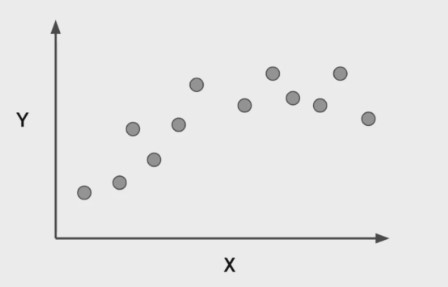
\includegraphics[scale=.5]{img/overfitting1.jpg}}
\end{figure}
	So here we have a bunch of training points and so there's some single feature X and at the end of the day we want to build out a model that can predict Y.
	
	 so a good model would try to fit the general trend pf the actual data set here so we can see it appears that there's some sort of positive slope and it looks like it levels off later on!
\begin{figure}[htbp]
\centerline{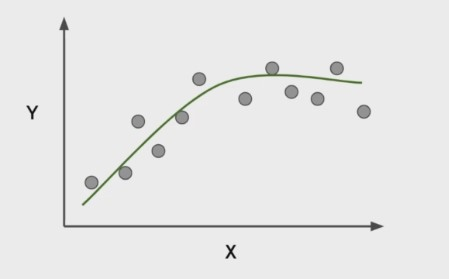
\includegraphics[scale=.5]{img/overfittingGoodModel.jpg}}
\end{figure}
 
	So what would happen if the model overfit to this training data, when you actually overfitting what's going to happen, you're actually going to fit too much to the noise of the data.
	\begin{figure}[htbp]
\centerline{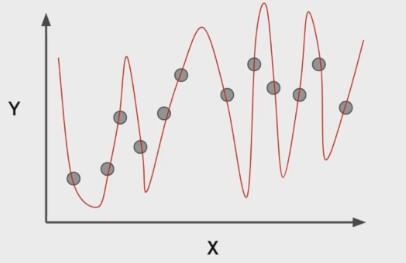
\includegraphics[scale=.5]{img/overfittingnoise.jpg}}
\end{figure}

	So here we have what appears to be a really bad model, but keep in mind that this model is technically hitting every single one of those training point. So your error here is actually going to be extremely low, and in this specific example your error is actually zero, because your model is accounting for every point in the every training set. So your error just on the training set is actually really low when you're overfitting. That's why it can be really deceptive and that's why we also need the validation and test sets in order to understand whether or not we're overfitting because just the training data alone won't tell us that information. 
	
	So, what happens when you're overfitting is your're fitting too much to the noise of the data here, if you were to get a new point and this would be a test or validation point if you're overfitting, that means you're getting low error on the training set, but when you get a new test so that the model hasn't seen before you're going to get a much larger error of your model.
		\begin{figure}[htbp]
\centerline{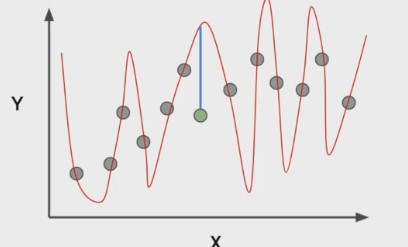
\includegraphics[scale=.5]{img/overfittingLargerError.jpg}}
\end{figure}


	\item 
	\section{Underfitting}
	
	\begin{itemize}
		\item
		Model does not capture the underlying trend of the data and does not fit the data well enough.
		\item
	Low variance but high bias.		
		\item
	Underfitting is often a result of an excessively simple model.
	\end{itemize}

	So in that same situation if we were to have the feature X and the label Y something that was underfitting 
	would just not even be able to grab the general trend! So maybe it picks up on that first upward slope but doesn't really grasp the idea that this model should eventually level off for the value of increase X.
	
\begin{figure}[htbp]
\centerline{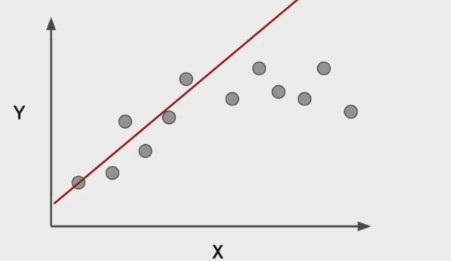
\includegraphics[scale=.5]{img/underfittingUpwardSlope.jpg}}
\end{figure}
	
	\LARGE Important Section to Learn!
	
	\small
	\begin{itemize}
		\item
		This data was easy to visualize, but how can we see underfitting and overfitting when dealing with multi dimensional data sets?
		
		\item
		First let's imagine we trained a model and then measured its error over training time.
	\end{itemize}
	
	\Large Let's imagine we have what should be a good model.
	\begin{figure}[htbp]
\centerline{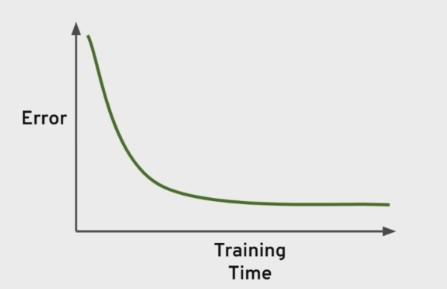
\includegraphics[scale=.5]{img/underfittingGoodModel.jpg}}
\end{figure}
	\small
	Well, as you can imagine a good model when it first encounters the training data it's going to have a large of error, because it hasn't actually seen this data before and has adjust any internal parameters to this data! However as you train your model for more time on the training data you would expect the error to essentially go down until it levels off and converge to some sort of minimum error. So this is what a good model should look like.
	
	 When we're specifically talking about neural networks this training time actually has a specific word and depending if you pronounce it the American way which is "epic" or British way "epoch" which is the way i pronounce (because my main language is not English, but well i try to pronounce epoch) it essentially one epoch the entirely of your training data one time trough your model.
	
	let's imagine a bad model.
	
	\begin{figure}[htbp]
\centerline{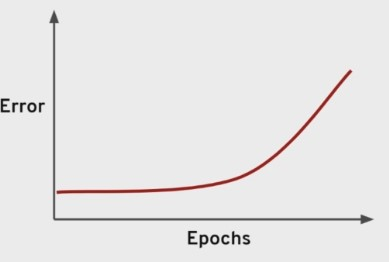
\includegraphics[scale=.5]{img/underfittingBadModel.jpg}}
\end{figure}
	
	If you train it for more and more time would get increasing error and that's not good because essentially your models not learning every time it goes thorough the train data it's actually increase error.
	
	\newpage
	\begin{itemize}
		\item

		\Large Let's imagine we split our data into a \textbf{training set} and a \textbf{test set}.
	\end{itemize}
	
	\small
	
	We first see performance on the training set.
\begin{figure}[htbp]
\centerline{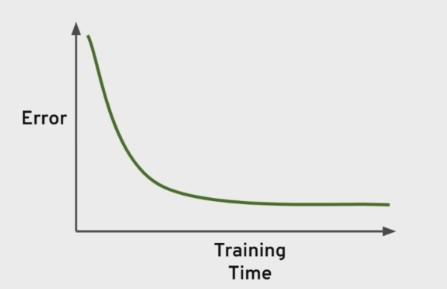
\includegraphics[scale=.5]{img/underfittingGoodModel.jpg}}
\end{figure}\\
	Typically you're training set performance is going to decrease in error as you train it for more epochs.\\
	
	Next we check the performance on the test set and is an ideal situation you will get similar behavior.
\begin{figure}[htbp]
\centerline{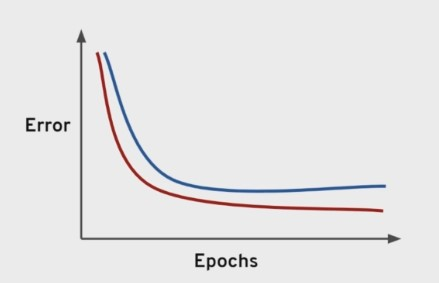
\includegraphics[scale=.5]{img/testset.jpg}}
\end{figure}\\

	The test set as you train for more epochs the training data then your error on the test set will also decrease. \newpage
	
	ideally the model would perform well on both with similar behavior. But what happens if we overfit on the training data? That means we would perform poorly on new test data!
	
\begin{figure}[htbp]
\centerline{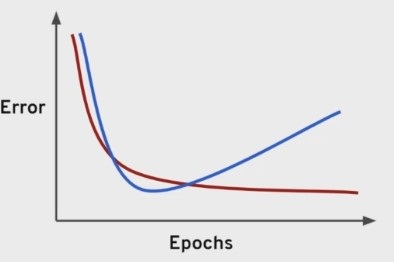
\includegraphics[scale=.5]{img/poorPerform.jpg}}
\end{figure}

	Red line as our training set and then that blue line as our test or validations set.\\
	
	So this is a good indication of training to much on that training dataset and you begin to overfitting. you have done too many passes on that training set and now your model can't generalize to data it hasn't seen before. it's only been able to predict now really well only on data it's seen.
	
	So what we want to do, is want to make sure we don't train too much on that specific training set, we can still generalize to new test or validation data and what we can do is we can plot out this behavior on the training set versus the test test set and then you should look to have a \textbf{cutoff point} on that training time, so as you can see the error on the test set start to increase, that's a good indication that's where \textbf{overfitting} on the training data would begin. So you want to kind of choose that cutoff point and it's not always as clear as this where essentially the intersect, but the main idea begin if you see an increase in error on that test set as the training error is still going down that's a good indication that you should stop training there.
\end{itemize}

\section{Evaluate Performance}
\subsection{Evaluating Performance Classification}

The key classification metrics we need to understand are:
\begin{itemize}
	\item
	\textbf{Accuracy}\\
		Accuracy in classification problems is the \textbf{number of correct predictions} made by the model divided by the \textbf{total number of prediction}.\\
		For example, if the X-test set was 100 images and our model correctly predicted 80 images, then we have 80/100 or \textbf{0.8} or \textbf{80\%}\textbf{ accuracy}.
	
	\begin{itemize}
		\item
		Accuracy is not a good choice with unbalanced classes!
		\item
		Imagine we had 99 images of dogs and 1 image of cat.
		\item
		If our model was simply a line that always predicted dog we would get 99\% accuracy.
	\end{itemize}
		
	\item
	\textbf{Recall}\\
		Ability of a model to find all the relevant(related) cases within a dataset.\\
		The precise definition of recall is the number of true positives \textbf{divided by} the number of true positives plus the number of false negative.
	\item
	\textbf{Precision}\\
	Ability of a classification model identify only the relevant data points.\\
	Precision is defined as the number of true positives divided by number of true positives plus the number of false positives.
	
	\item 
	\textbf{Recall and Precision:}\\
	Often you have a trade-off between Recall and Precision.\\
	While Recall, expresses the ability to find all relevant instance in a dataset.\\
	Precision, expresses the proportion of the data points our model says was relevant actually were relevant.
	\item
	\textbf{F1-Score}\\
	In cases where we want to find an optimal blend of precision and recall we can combine the two metrics using what is called the F1 Score.\\
	The F1 Score is the harmonic mean of precision and recall taking both metrics into account in the following equation:\\
	\begin{equation}
		F1 = 2 * \frac{precision * recall}{precision + recall}
	\end{equation}
\end{itemize}
But first, we should understand the reasoning behind these metrics and how thy will actually work in the real world!\\

typically in any classification task your model can only achieve two results:
\begin{itemize}
	\item
	Either your model was \textbf{correct} in its prediction.
	\item
	Or your model was \textbf{incorrect} in its prediction 
\end{itemize}


Fortunately incorrect vs correct expands to situations where you have multiple classes such as categories.\\
For the purposes of explaining the metrics, let's imagine a binary classification situation, where we only have two available classes(0, 1).\\


In my example, we will attempt to predict if an image is a dog or a cat.\\
Since this is supervised leaning, we will first \textbf{fit/train} a model on \textbf{training data}, then test the model on\textbf{ testing data}.\\
Once we have the model's predictions from the $x_test$ data, we compare it to the true y values (the correct labels.\\
\newpage

\LARGE
All of this is to say, ML is not performed in a "Vacuum", but instead a collaborative process where we should consult with experts in the domain (e.g.medical doctors)
\small

\subsection{Evaluating Performance Regression}
Let's take a moment now to discuss evaluating Regression Models.\\
	Regression is a task when a model attempts to predict continuous value (unlike categorical values, which is classification)
	You may have heard of some evaluation metrics like accuracy or recall.\\
	These sort of metrics aren't useful regression problems, we need metrics designed for continuous values.
 
 \begin{itemize}
 	\item
 	For example, attempting to predict the price of a house given its feature is a \textbf{regression task}.
 	\item
 	Attempting to predict the country a house is in given its features would be a classification task.
 \end{itemize}
 
 Let's discuss some of the most common evaluation metrics for regression:
 \begin{itemize}
 	\item
 	Mean Absolute Error
 	\item
 	Mean Squared Error
 	\item
 	Root Mean Square Error
 \end{itemize}
 
 
  \begin{itemize}
 	\item
 	\textbf{Mean Absolute Error (MAE):}\\
 	This is the mean of the absolute value of errors.\\
 	Easy to understand.
	\begin{equation}
		\frac{1}{n} \sum_{i=1}^{n} \mid y_{i}- y^{\wedge}_{i}\mid
	\end{equation}	 	

 	\item
 	\textbf{Mean Squared Error(MSE):}\\
 		Larger errors are noted more than with MAR, making MSE more popular.
		\begin{equation}
		 	\frac{1}{n} \sum_{i=1}^{n} (y_{i}- y^{\wedge}_{i})^{2}
		\end{equation}
 	\item
 	\textbf{Root Mean Square Error (RMSE) :}\\
 	Most popular (has same units as y)
 	\begin{equation}
	\sqrt{\frac{1}{n} \sum_{i=1}^{n} (y_{i}- y^{\wedge}_{i})^{2}}
 	\end{equation}
 \end{itemize}
 
\section{Unsupervised Learning}
 
 We've covered supervised learning, where the \textbf{label was known} due to \textbf{historical labeled data}.\\
 But what happens when we don't have historical labels?\\
 There are certain tasks that fall under Unsupervised Learning:
 \begin{itemize}
 	\item
 	Clustering 
 	\item
 	Anomaly Detection
 	\item
 	Dimensionality Reduction
\end{itemize} 

 \begin{itemize}
 	\item
 	\textbf{Clustering:}
	\begin{itemize}
		\item
		 		Grouping together \textbf{unlabeled} data points into categories/clusters
		 		
		 \item
		 Data points are assigned to a cluster based on similarity.
	\end{itemize}	 
 		
 	\item
 	\textbf{Anomaly Detection:}
 	\begin{itemize}
 		\item
 		Attempts to detect outliers in a dataset
 		\item
 		For example, fraudulent transactions on a credit card.
 	\end{itemize}
 	\item
 	\textbf{Dimensionality Reduction:}
 	\begin{itemize}
 		\item
 		Data processing the techniques that reduces the number of features in a data set, either for compression, or to better understand underlying trends with in a data set.
 	\end{itemize}
\end{itemize} 

Unsupervised Learning:\\
it's important to note, these are situations where we \textbf{don't} have the correct answer for historical data.\\
\large which means evaluation is much harder and more nuanced!
\small

\section{Artificial Neural Networks}

\subsection{Perceptron model}
To begin understanding deep learning,m we will build up our model abstractions:\\
\begin{itemize}
	\item
	Single Biological Neuron
	\item
	Preceptron 
	\item
	Multi-layer Perceptron Model
	\item
	Deep Leaning Neural Network
\end{itemize}

\begin{figure}[htbp]	\centerline{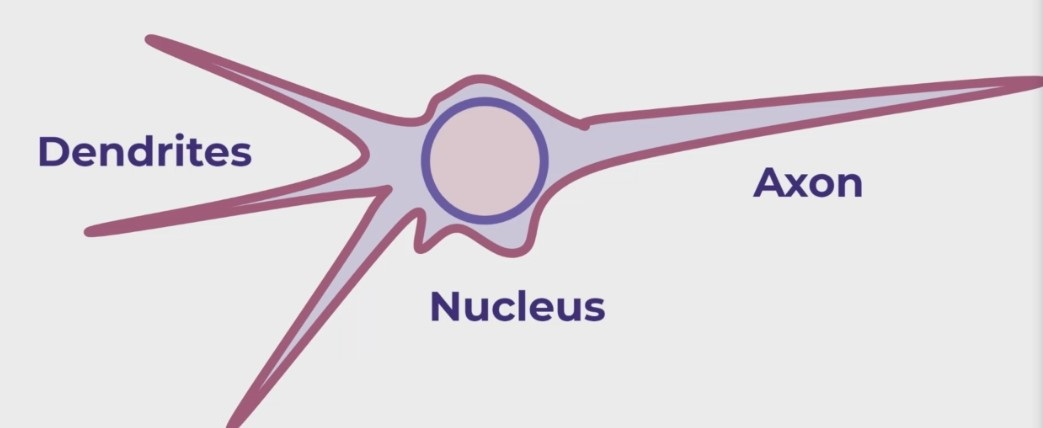
\includegraphics[scale=.5]{img/biologicalNN.jpg}}
	\caption{Simplified Biological Neuron Model(3 input $\rightarrow$ 1 output)}
\end{figure}


A \textbf{perceptron} was a form of neural network introduced in 1958 by Frank Rosenblatt.\\
Amazingly, even back then he saw huge potential:\\
\large "\textbf{Perceptron} may eventually be able to learn, make decisions, and translate languages."
\small\\
\newpage
\textbf{If f(x) is just a sum, then y=x1+x2}
\begin{figure}[htbp]	\centerline{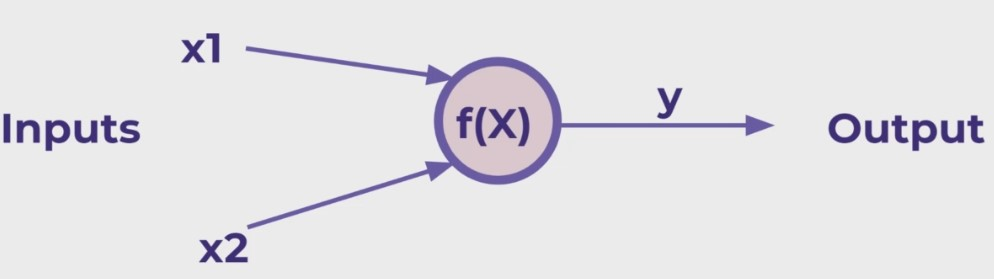
\includegraphics[scale=.5]{img/sumPerceptron.jpg}}
\end{figure}
\newpage



To build a network of perceptrons, we can connect layers of perceptrons, using a \textbf{multi-layer perceptron model}. The outputs of one perceptron are directly fed into as inputs to another perceptron.
\begin{figure}[htbp]	\centerline{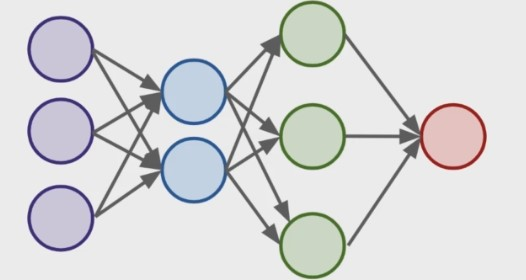
\includegraphics[scale=.5]{img/multiPerceptronModel.jpg}}
\end{figure}

The fist layer is the input layer, can be a series of categories or some data points or tabular of data as input to this perceptron model.
\begin{figure}[htbp]	\centerline{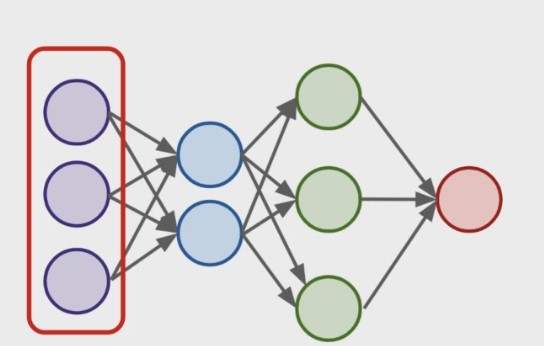
\includegraphics[scale=.5]{img/inputLayer.jpg}}
\end{figure}

The last layer is the output layer.\\
\textbf{NOTE}: This last layer can be more than one neuron.
\begin{figure}[htbp]	\centerline{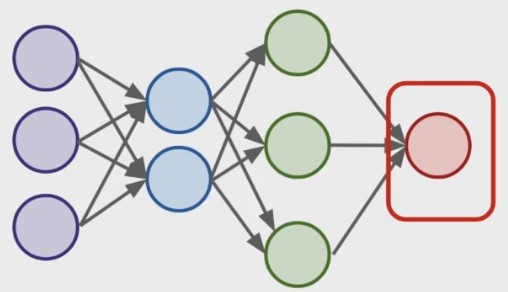
\includegraphics[scale=.5]{img/outputLayer.jpg}}
\end{figure}

Hidden layers are difficult to interpret, due to their high interconnectivity and distance away from known input or output values.
\begin{figure}[htbp]	\centerline{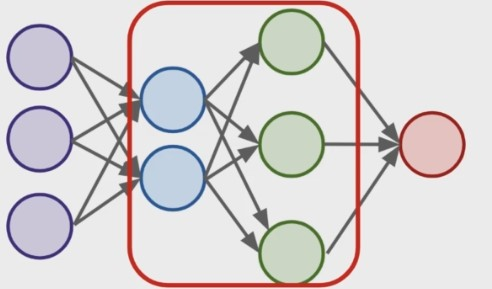
\includegraphics[scale=.5]{img/hiddenLayer.jpg}}
\end{figure}

Neural Networks become "Deep neural networks" if then contain 2 or more \textbf{hidden layers}.
\begin{figure}[htbp]	\centerline{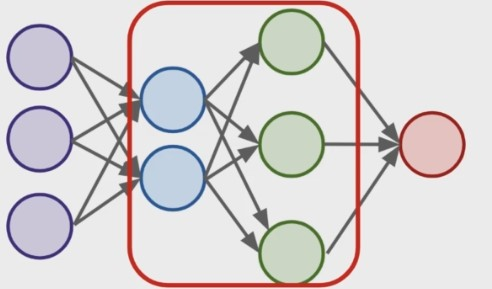
\includegraphics[scale=.5]{img/hiddenLayer.jpg}}
\end{figure}


\begin{figure}[htbp]	\centerline{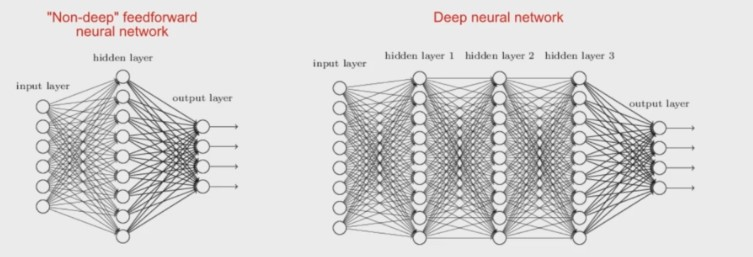
\includegraphics[scale=.52]{img/deep_and_none_deep.jpg}}
\caption{Deep and non deep neural networks}
\end{figure}
\newpage

\Large Terminology:\small
\begin{itemize}
	\item
	\textbf{Input Layer:} First layer that directly accepts real data values.
	\item
	\textbf{Hidden Layer:} Any layer between input and output layers.
	\item
	\textbf{Output Layer:} The final estimate of the output.
\end{itemize}



















\end{document}